\documentclass[11pt,letterpaper]{article}
\usepackage[latin1]{inputenc}
\usepackage{amsmath}
\usepackage{amsfonts}
\usepackage{amssymb}
\usepackage{graphicx}
\usepackage{capt-of}

\setlength{\parskip}{1pc}
\setlength{\parindent}{0pt}
\setlength{\topmargin}{-3pc}
\setlength{\textheight}{9.0in}
\setlength{\oddsidemargin}{0pc}
\setlength{\evensidemargin}{0pc}
\setlength{\textwidth}{6.5in}

\title{6.170 Assignment 2: Object Models}
\author{Dina Betser}


\begin{document}
\maketitle

\section{Background}
\begin{enumerate}
\item Entity Relationship Model\\
ER modeling is used to describe the type of information that is to be stored in a database. Objects are represented as ``entities''.
\item Object Modeling Technique\\
This was developed as a method to develop object-oriented systems and to support OOP. Objects and their relationships are expressed using multiplicities.
\item Software Analysis Patterns\\
This modeling technique aims to represent ideas that have been useful in one practical context and will probably be useful in others.
\item Unified Modeling Language\\
The most sophisticated of the languages listed, UML is a standard modeling language that has a lot of the same characteristics as the object modeling notation used in this class, including inheritance.
\end{enumerate}

One feature that is present in all modeling formats except for ER modeling is inheritance/generalization.

\section{Conceptual modeling problems}
\begin{itemize}
\item Prerequisites. Model the relationships between classes and their prerequisites. Note that there may be different ways in which the prerequisites of a class can be satisfied; for example, two prerequisite classes may be interchangeable.\\

\begin{enumerate}
\item Ambiguities Resolved\\
The fact that multiple combinations of prerequisites can satisfy the prerequisites of a given class was disambiguated by creating a ``Prerequisite Set'' entity, which encapsulates the Boolean logic of (class1 and class2) OR (class3 and class1). The Prerequisite Set for any Class enumerates all of these possible combinations.

\item Complexities Ignored\\
Assumed that there were no other types of ways to get Credit for a class other than those listed.

\item Designations\\
A \texttt{Credit} is defined as some form of knowledge that satisfies a given prerequisite. This could be in the form of transfer credit from another school, an Advanced Standing Exam that was taken successfully, or having taken the Classes at the same school with passing grades.


\item Object Model\\
\begin{center}
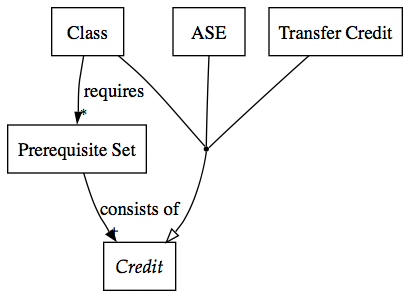
\includegraphics[width=300pt]{dot/b1.png}
\label{fig:ob1} 
\end{center}
\end{enumerate}

\item Street map. Model a street map that includes named streets and their intersections, and the notion of one-way streets and divided highways. Note in particular that one street may be accessible from an intersecting street only for traffic moving in a particular direction.

\begin{enumerate}
\item Ambiguities Resolved\\
I differentiated between Highway-type streets (both divided and undivided), and Non-Highway (``Named'') Streets (both one way and two-way). Intersections happen between named streets only, while Highways intersect with both other Highways and Streets using Ramps.
\item Complexities Ignored\\
The idea of accessibility is briefly included as the idea that Streets have a Direction which allows them to access other Streets, but beyond that, further complexity was ignored. For instance, the fact that a one-way Street only has one Direction is not specified.
\item Designations\\
A Street is a complex concept. It might better be referred to as a ``half-street''. Every ``Street'' is associated with a Direction, or cardinality. This, for two-way streets, means that each street has an Up or Down direction, just like electron spin. :)

\item Object Model\\
\begin{center}
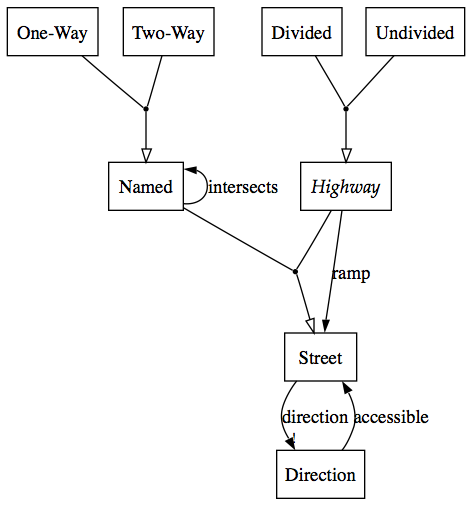
\includegraphics[width=300pt]{dot/b2.png}
\label{fig:ob2} 
\end{center}
\end{enumerate}

\item Voting ballots. Model the ballots cast in a voting scheme, in which on each ballot the voter makes choices of candidates for a variety of offices.

\begin{enumerate}
\item Ambiguities Resolved\\
It was ambiguous whether or not to include a Voter in the model, but I chose to in order to represent that there is a person behind any Ballot that is cast.
\item Complexities Ignored\\
Different voting schemes can be supported by this object model, since every Voter always makes a set of selections, which are merely tuples of the Office and the Candidate. This can support things like ``Pick 2'' elections where every Voter selects two Candidates for a given Office. However, the model is overly flexible in that it does not prevent Voters from selecting a Candidate who is not running for a given Office.
\item Designations\\
A Ballot is designated as an Entity that includes a race for multiple Offices, each of which consists of one or more Candidates. 
A Selection is a tuple of (Office, Candidate).
\item Object Model\\
\begin{center}
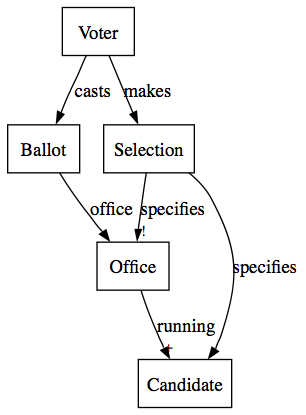
\includegraphics[width=200pt]{dot/b3.png}
\label{fig:ob3} 
\end{center}
\end{enumerate}

\item Java types. Model the type structure of objects in a Java program, in which there are two kinds of types, class types and interfaces, related by implements and extends. Include in your model a notion of variables, each with a declared type and containing an object of a given type. What is the relationship between the two types?\\

\begin{enumerate}
\item Ambiguities Resolved\\
In Java, all Classes, Interfaces, and Variables have a Type. However, variables have a declared type (static) and a type at runtime (dynamic type) which depends on how the Variable is defined and initialized. The dynamic type is always a subclass of the static type.
\item Complexities Ignored\\
I ignored the concept of Primitives as recommended in the problem statement; if they had been included, it would be as another disjoint subset of Type.
\item Designations\\
The extends/implements relationships were taken directly from the Java documentation to ensure that Classes and Interfaces can be extended as appropriate.
The idea of an Object was introduced in order to allow a Variable to take on a more specific runtime type than the static type with which it was declared.
\item Object Model\\
\begin{center}
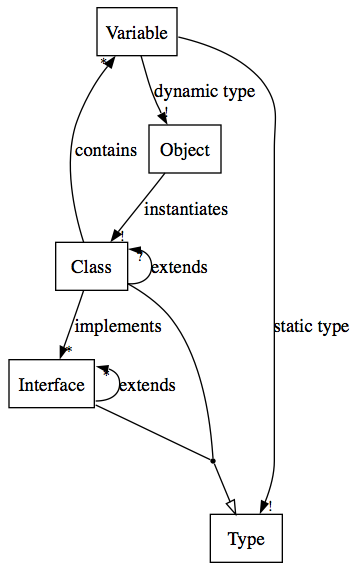
\includegraphics[width=200pt]{dot/b4.png}
\label{fig:ob4} 
\end{center}
\end{enumerate}

\end{itemize}



\section{Modeling Python Modules}
\begin{enumerate}
\item Ambiguities Resolved\\
The Python Path is a singleton item since it refers to an ordered list of directories from which the Python interpreter can retrieve Python modules. Every Module has a ``path'', which is a Directory, but every Module Name can be associated with multiple Files. However, the combination of a Directory path and Module name uniquely identifies a file.
\item Complexities Ignored\\
The idea of a ``current'' symbol table for the ``current'' Python module is something I thought about but decided to leave out, since for any Module, import statements can change the Symbol table associated with that module.
\item Designations\\
In this problem, a ``Symbol Table'' maintains a set of ``Entry''s, and Python modules add tuples to this table. The two types of import statements work differently in that \texttt{from mod import *} adds $n$ elements to the symbol table, where $n$ is the number of elements in the module. The statement \texttt{import mod} merely adds the mod element to the symbol table, and all the symbols from that module can be accessed via that module's entry.
\item Object Model\\
\begin{center}
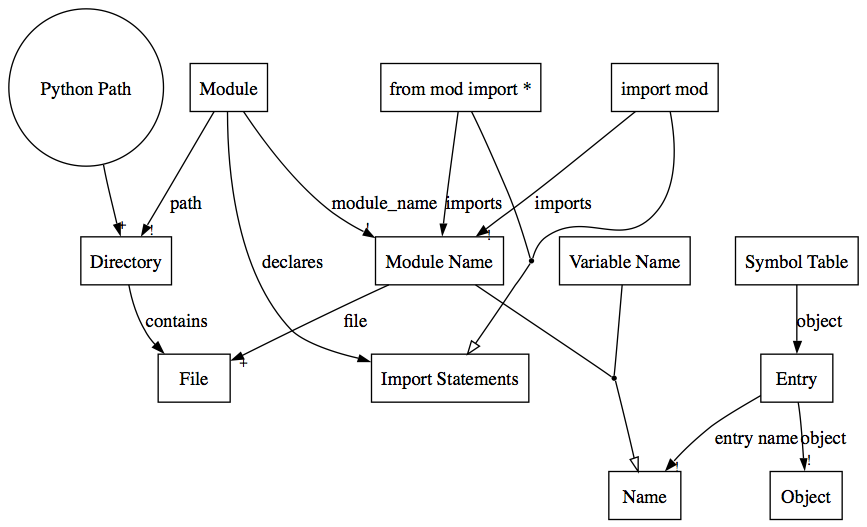
\includegraphics[width=500pt]{dot/pythonmodules.png}
\label{fig:ob5}
\end{center}
\end{enumerate}

\section{Extracting an OM from an API}
\begin{enumerate}
\item Ambiguities Resolved\\
It was unclear whether the three items (Callback, etc.) were really data sources or an API to retrieve data. I ended up naming the entity from which they descend a ``Source Option'' to specify that they were a method of generating data.
\item Complexities Ignored\\
The complexities inherent in the way the 3 source options can be used were ignored and encapsulated by just referring to the name of the method.
\item Designations\\
The ``Result Set'' refers to the data generated when a ``Search Term'' is entered into the ``Autocomplete Instance''.
\item Object Model\\
\begin{center}
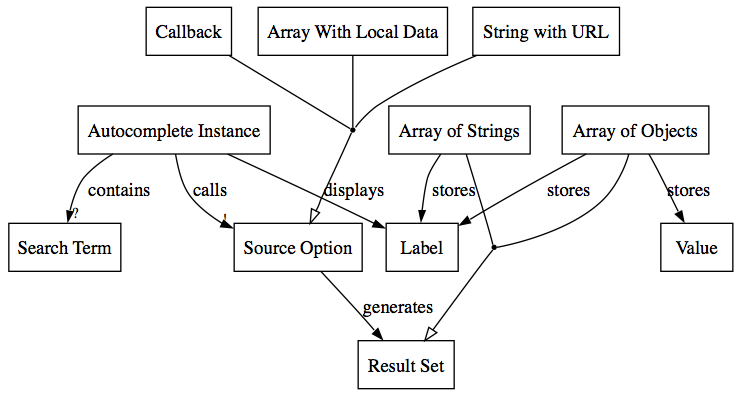
\includegraphics[width=400pt]{dot/autocomplete.png}
\label{fig:ob6} 
\end{center}
\end{enumerate}

\section{Metamodeling}
\begin{enumerate}
\item Ambiguities Resolved\\
It was ambiguous whether the ``disjoint set'' relationship referred to the parent-child subset relationship, or among children in a parent-child subset relationship. I chose to assume the latter, so Sets are described as disjoint with respect to other sets.

\item Complexities Ignored\\
In the modified version of the metamodeling object model, I've created a ``disjoint tree'' entity to encapsulate the entities of a subset relation with its parent and disjoint children.
\item Designations\\
A Multiplicity refers to the type of multiplicity that a Set or Relation may have; I've included the shorthand notation instead of the term such as ``?'' to stand in for ``0 or 1''.
A Singleton set is always represented with an oval instead of a rectangle.
\item Object Models\\
Part 1:
\begin{center}
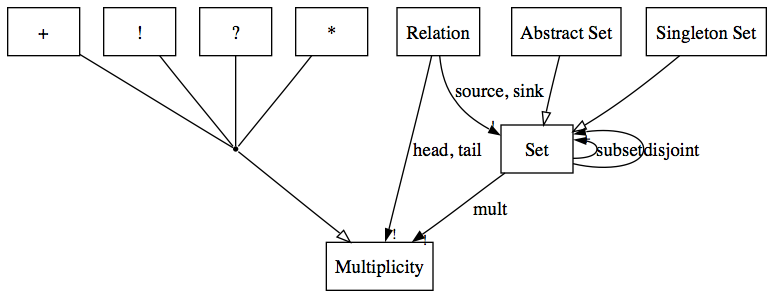
\includegraphics[width=400pt]{dot/metamodeling.png}
\label{fig:ob7} 
\end{center}

Part 2:
The extension is to include a new character (in this case, an @ symbol) where the subsets attached to an inheritance arrow are exhaustive.

The new version of the object model is below in Figure \ref{fig:ob8}.

\begin{center}
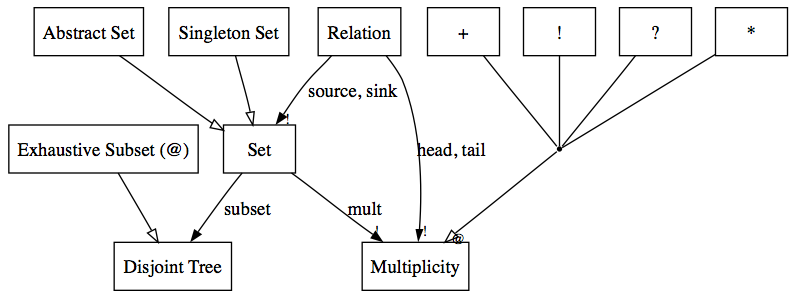
\includegraphics[width=400pt]{dot/metamodeling2.png}
\label{fig:ob8} 
\end{center}

In the diagram in Figure \ref{fig:ob8}, the only exhaustive relation is the symbols that subclass the Multiplicity entity, so as such, an @ symbol is attached to the open arrowhead.

There are pros and cons to specifying exhaustive sets in this manner. The plus side is that an exhaustive relation should really be designed in the relation itself, not in the set that is being subset. However, adding this to the notation adds another layer of complexity which may not necessarily be a good idea. The current object modeling schematic makes the design decision to leave such notation out, and as such it gains in simplicity what it might have lost in expressiveness. These types of design decisions must be made, and given the not-so-frequent cases that 


\end{enumerate}

\end{document}

